\section{Method}
\label{Met}
\subsection{Overall architecture}
\label{sec:method}
Inspired by the two-branch architectures~\cite{yu2021bisenet, poudel2019fast, hong2021deep,huang2021alignseg,chen2022mobile}, we design a {\bf s}queeze-{\bf e}nhanced {\bf A}xial Trans{\bf former} ({\bf SeaFormer}) framework. 
As is shown in Figure~\ref{fig:pipeline}, SeaFormer consists of these parts: \textit{shared STEM}, \textit{context branch}, \textit{spatial branch}, \textit{fusion block} and \textit{light segmentation head}.
For a fair comparison, we follow TopFormer~\cite{zhang2022topformer} to design the STEM. 
It consists of one regular convolution with stride of 2 followed by four MobileNet blocks where stride of the first and third block is 2.
The context branch and the spatial branch share the produced feature map,  which allows us to build a fast semantic segmentation model.

\subsubsection{Context branch}
The context branch is designed to capture context-rich information from the feature map $\mathbf{x}_s$.
As illustrated in the red branch of Figure~\ref{fig:pipeline}, the context branch is divided into three stages.
To obtain larger receptive field, we stack SeaFormer layers after applying a MobileNet block to down-sampling and expanding feature dimension. 
Compared with the standard convolution as the down-sampling module, MobileNet block increases the representation capacity of the model while maintaining a lower amount of computation and latency.
For variants except SeaFormer-Large, SeaFormer layers are applied in the last two stages for superior trade-off between accuracy and efficiency. 
For SeaFormer-Large, we insert SeaFormer layers in each stage of context branch.
To achieve a good trade-off between segmentation accuracy and inference speed, we design a squeeze-enhanced Axial attention block (SEA attention) illustrated in the next subsection.

\begin{figure*}
  % \vspace{-0.7cm}
  \centering
  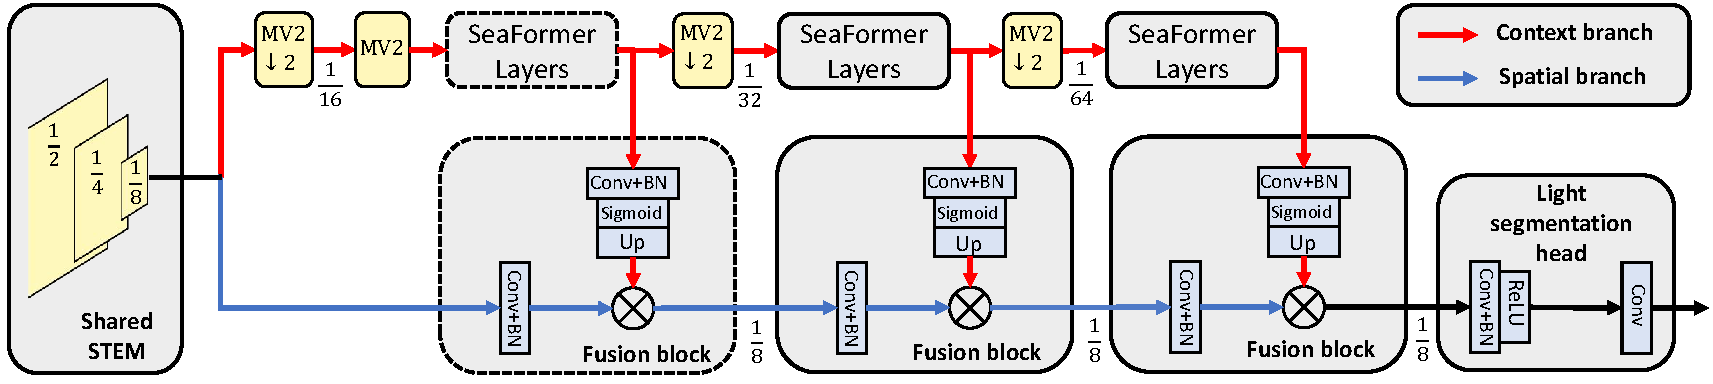
\includegraphics[width=\hsize]{pipeline_.pdf}
  \caption{The overall architecture of SeaFormer. It contains shared STEM, context branch (\textbf{red}), spatial branch (\textbf{blue}), fusion block and light segmentation head. 
  \texttt{MV2} block means MobileNetV2 block and \texttt{MV2} {$\downarrow$}2 means MobileNetV2 block with downsampling. 
  SeaFormer layers and fusion block with dash box only exist in SeaFormer-L. The symbol
  $\bigotimes$ denotes element-wise multiplication.
  }
  \label{fig:pipeline}
  % \vspace{-0.2cm}
\end{figure*}
\subsubsection{Spatial branch}
The spatial branch is designed to obtain spatial information in high resolution. 
Identical to the context branch, the spatial branch reuses feature maps $\mathbf{x}_s$. 
However, the feature from the early convolution layers contains rich spatial details but lacks high-level semantic information. 
Consequently, we design a fusion block to fuse the features in the context branch into the spatial branch, bringing high-level semantic information into the low-level spatial information.

\subsubsection{Fusion block}
As depicted in Figure~\ref{fig:pipeline}, high resolution feature maps in the spatial branch are followed by a 1 × 1 convolution and a batch normalization layer to produce a feature to fuse. 
Low resolution feature maps in the context branch are fed into a $1 \times 1$ convolution layer, a batch normalization layer, a sigmoid layer and up-sampled to high resolution to produce semantics weights by bilinear interpolation. 
Then, the semantics weights from context branch are element-wisely multiplied to the high resolution feature from spatial branch.
The fusion block enables low-level spatial features to obtain high-level semantic information.

\subsubsection{Light segmentation head}
The feature after the last fusion block is fed into the proposed segmentation head directly, as demonstrated in Figure~\ref{fig:pipeline}. 
For fast inference purpose, our light segmentation head consists of two convolution layers, which are followed by a batch normalization layer separately and the feature from the first batch normalization layer is fed into an activation layer.

\subsection{Squeeze-enhanced Axial attention}
\label{sec:sea_attn}
The global attention can be expressed as 
\begin{equation}
    \mathbf{y}_o = \sum_{p\in \mathcal{G}(o)} \text{softmax}_p\left(\mathbf{q}_o^\top \mathbf{k}_p \right)\mathbf{v}_p
\end{equation}
where $\mathbf{x}\in \mathbb{R}^{H\times W\times C}$. $\mathbf{q,k,v}$ are linear projection of $\mathbf{x}$, \ie $\mathbf{q}=\mathbf{W}_q\mathbf{x}, \mathbf{k}=\mathbf{W}_k\mathbf{x}, \mathbf{v}=\mathbf{W}_v\mathbf{x}$, where $\mathbf{W}_q, \mathbf{W}_k\in \mathbb{R}^{C_{qk}\times C}, \mathbf{W}_v\in \mathbb{R}^{C_v\times C}$ are learnable weights. $\mathcal{G}(o)$ means all positions on the feature map of location $o=(i, j)$.
When traditional attention module is applied on a feature map of $H\times W\times C$, the time complexity can be $\mathcal{O}(H^2 W^2(C_{qk}+C_v))$, leading to low efficiency and high latency. 

\begin{align}
    \label{equ:nei_attn} \mathbf{y}_o &= \sum_{p\in \mathcal{N}_{m\times m}(o)}\text{softmax}_p\left(\mathbf{q}_o^\top \mathbf{k}_p \right)\mathbf{v}_p
\end{align}
\begin{equation}
\begin{split}
    \label{equ:axial_attn} \mathbf{y}_o = \sum_{p\in \mathcal{N}_{1\times W}(o) }\text{softmax}_p\left(\mathbf{q}_o^\top \mathbf{k}_p \right)\mathbf{v}_p \\
    ~~~+ \sum_{p\in \mathcal{N}_{H\times 1}(o) }\text{softmax}_p\left(\mathbf{q}_o^\top \mathbf{k}_p \right)\mathbf{v}_p
\end{split}
\end{equation}

To improve the efficiency, there are some works~\cite{liu2021swin,huang2019ccnet,ho2019axial} computing self-attention within the local region. 
We show two most representative efficient Transformer in Equation~\ref{equ:nei_attn},~\ref{equ:axial_attn}.
Equation~\ref{equ:nei_attn} is represented by window-based attention~\cite{luong2015effective} successfully reducing the time complexity to $\mathcal{O}(m^2HW(C_{qk}+C_v))=\mathcal{O}(HW)$, where $\mathcal{N}_{m\times m}(o)$ means the neighbour $m\times m$ positions of $o$, but loosing global receptiveness.
The Equation~\ref{equ:axial_attn} is represented by Axial attention~\cite{ho2019axial}, which only reduces the time complexity to $\mathcal{O}((H+W)HW(C_{qk}+C_v))=\mathcal{O}((HW)^{1.5})$, where $\mathcal{N}_{H\times 1}(o)$ means all the positions of the column of $o$; $\mathcal{N}_{1\times W}(o)$ means all the positions of the row of $o$.

According to their drawbacks, we propose the mobile-friendly squeeze-enhanced Axial attention, with a succinct squeeze Axial attention for global semantics extraction and an efficient convolution-based detail enhancement kernel for local details supplement.
\begin{equation}
\begin{split}
\label{equ:hori_ver_squ}
    \mathbf{q}_{(h)} = \frac{1}{W}\left(\mathbf{q}^{\rightarrow(H,C_{qk}, W)}\mathbf{A}_W^{\rightarrow(H,W,1)}\right)^{\rightarrow(H, C_{qk})} \\
    \mathbf{q}_{(v)} = \frac{1}{H}\left(\mathbf{q}^{\rightarrow(W, C_{qk}, H)}\mathbf{A}_H^{\rightarrow(W,H,1)}\right)^{\rightarrow(W, C_{qk})}
    \end{split}
\end{equation}

\subsubsection{Squeeze Axial attention}
To achieve a more efficient computation and aggregate global information at the same time, we resort to a more radical strategy.
In the same way, $\mathbf{q},\mathbf{k},\mathbf{v}$ are first get from $\mathbf{x}$ with $\mathbf{W}_q^{(s)}, \mathbf{W}_k^{(s)}\in \mathbb{R}^{C_{qk}\times C}, \mathbf{W}_v^{(s)}\in \mathbb{R}^{C_v\times C}$.
According to Equation~\ref{equ:hori_ver_squ}, we first implement \textit{horizontal squeeze} by employing an input adaptive approach, using a learnable mask to map all tokens of query to a single token in each row.
In the same way, the second row of the equation shows the \textit{vertical squeeze} in the vertical direction.
$\mathbf{z}^{\rightarrow(\cdot)}$ means permuting the dimension of tensor $\mathbf{z}$ as given, and $\mathbf{A}$ is a learnable mask that is adaptively adjusted according to the input feature $\mathbf{x}$. It is formed by applying a 1 $\times$ 1 convolution and batch normalization layer on the input feature map \textbf{x}
The adaptive squeeze operation on $\mathbf{q}$ also repeats on $\mathbf{k}$ and $\mathbf{v}$, so we finally get $\mathbf{q}_{(h)}, \mathbf{k}_{(h)}, \mathbf{v}_{(h)}\in\mathbb{R}^{H\times C_{qk}}$, $\mathbf{q}_{(v)}, \mathbf{k}_{(v)}, \mathbf{v}_{(v)}\in\mathbb{R}^{W\times C_{qk}}$.
The squeeze operation reserves the global information to a single axis in an adaptive manner, thus greatly alleviating the following global semantic extraction shown by Equation~\ref{equ:saa}.
\begin{equation}
\begin{split}
\label{equ:saa}
    \mathbf{y}_{(i,j)} = \sum_{p=1}^{H}\text{softmax}_p\left( \mathbf{q}_{(h)i}^\top \mathbf{k}_{(h)p} \right)\mathbf{v}_{(h)p}\\
    + \sum_{p=1}^W\text{softmax}_p\left( \mathbf{q}_{(v)j}^\top \mathbf{k}_{(v)p} \right)\mathbf{v}_{(v)p}
\end{split}
\end{equation}
Each position of the feature map propagates information only on two squeezed axial features.
Similar to adaptive squeezing operation, a 1 $\times$ 1 convolution and batch normalization layer is used to generate an input-adaptive mask for feature restoration. The detail is shown in Figure~\ref{fig:squeeze_expand}. Compared with the pooling operation for squeezing and broadcast for expanding, the adaptive squeezing and expanding operations help the model aggregate spatial information in an input-adaptive way without introducing excessive computational overhead. The empirical study confirms the effectiveness of the approach.
Time complexity for adaptive squeezing $\mathbf{q},\mathbf{k},\mathbf{v}$ is $\mathcal{O}(HW(2C_{qk}+C_v))$, the attention operation takes $\mathcal{O}((H^2+W^2)(C_{qk}+C_v))$ time and the adaptive expanding takes $\mathcal{O}(HW(2C_{qk}+C_v))$ time.
Thus, our squeeze Axial attention successfully reduces time complexity to $\mathcal{O}(HW)$. 

\subsubsection{Squeeze Axial position embedding} Equation~\ref{equ:hori_ver_squ} are, however, not positional-aware, including no positional information of the feature map.
Hence, we propose squeeze Axial position embedding to squeeze Axial attention.
For squeeze Axial attention, we render both $\mathbf{q}_{(h)}$ and $\mathbf{k}_{(h)}$ to be aware of their position in the squeezed axial feature by introducing positional embedding $\mathbf{r}_{(h)}^{q}, \mathbf{r}_{(h)}^{k}\in \mathbb{R}^{H\times C_{qk}}$, which are linearly interpolated from learnable parameters $\mathbf{B}_{(h)}^{q}, \mathbf{B}_{(h)}^{k}\in \mathbb{R}^{L\times C_{qk}}$.
$L$ is a constant.
In the same way, $\mathbf{r}_{(v)}^q, \mathbf{r}_{(v)}^k\in \mathbb{R}^{W\times C_{qk}}$ are applied to $\mathbf{q}_{(v)}, \mathbf{k}_{(v)}$.
Thus, the positional-aware squeeze Axial attention can be expressed as Equation~\ref{equ:saa_pos}.
\begin{figure*}
  % \vspace{-0.7cm}
  \centering
   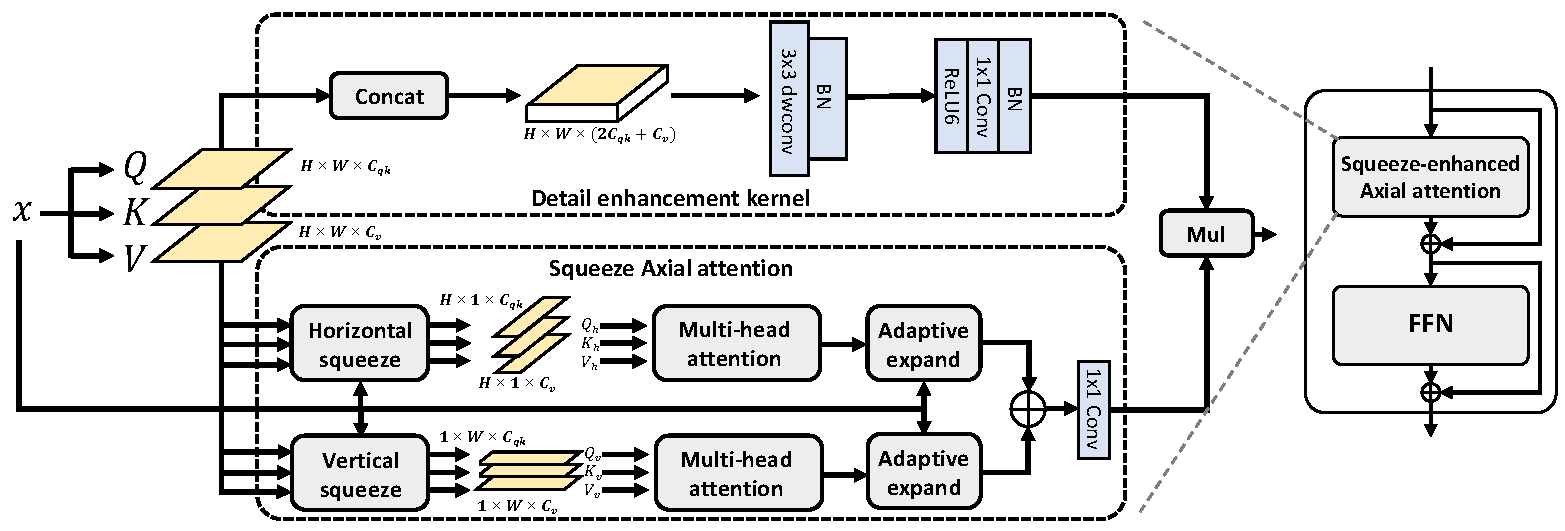
\includegraphics[width=\hsize]{sea_transformer.pdf}
  \caption{\textit{\textbf{Right}}: the schematic illustration of the proposed squeeze-enhanced Axial Transformer layer including a squeeze-enhanced Axial attention and a Feed-Forward Network (FFN).
  \textit{\textbf{Left}} is the squeeze-enhanced Axial Transformer layer, including detail enhancement kernel and squeeze Axial attention. The symbol $\bigoplus$ indicates an element-wise addition operation. Mul means multiplication.
  }
  \label{fig:transformer}
  % \vspace{-0.2cm}
\end{figure*}
\begin{equation}
\begin{split}
\label{equ:saa_pos}
    \mathbf{y}_{(i,j)} = \sum_{p=1}^{H}\text{softmax}_p\left((\mathbf{q}_{(h)i} + \mathbf{r}_{(h)i}^{q})^\top (\mathbf{k}_{(h)p} + \mathbf{r}_{(h)p}^{k})\right)\mathbf{v}_{(h)p}\\
    + \sum_{p=1}^W\text{softmax}_p\left((\mathbf{q}_{(v)j} + \mathbf{r}_{(v)j}^{q})^\top (\mathbf{k}_{(v)p} + \mathbf{r}_{(v)p}^{k}) \right)\mathbf{v}_{(v)p}
\end{split}
\end{equation}


\subsubsection{Detail enhancement kernel}
The squeeze operation, though extracting global semantic information efficiently, sacrifices the local details. 
Hence an auxiliary convolution-based kernel is applied to enhance the spatial details. 
As is shown in the upper path of Figure~\ref{fig:transformer}, $\mathbf{q},\mathbf{k},\mathbf{v}$ are first get from $\mathbf{x}$ with another $\mathbf{W}_q^{(e)}, \mathbf{W}_k^{(e)}\in \mathbb{R}^{C_{qk}\times C}, \mathbf{W}_v^{(e)}\in \mathbb{R}^{C_v\times C}$ and are concatenated on the channel dimension and then passed to a block made up of 3$\times$3 depth-wise convolution and batch normalization. 
By using a 3$\times$3 convolution, auxiliary local details can be aggregated from 
$\mathbf{q},\mathbf{k},\mathbf{v}$. 
And then a linear projection with activation function and batch normalization is used to squeeze $(2C_{qk}+C_{v})$ dimension to $C$ and generate detail enhancement weights.
Finally, the enhancement feature will be fused with the feature given by squeeze Axial attention. 
Different enhancement modes including element-wise addition and multiplication will be compared in the experiment section.
Time complexity for the 3$\times$3 depth-wise convolution is $\mathcal{O}(3^2HW (2C_{qk}+C_v))$ and the time complexity for the 1$\times$1 convolution is $\mathcal{O}(HWC(2C_{qk}+C_{v}))$. 
Time for other operations like activation can be omitted.

\begin{figure}[tb]
  % \vspace{-0.7cm}
  \centering
   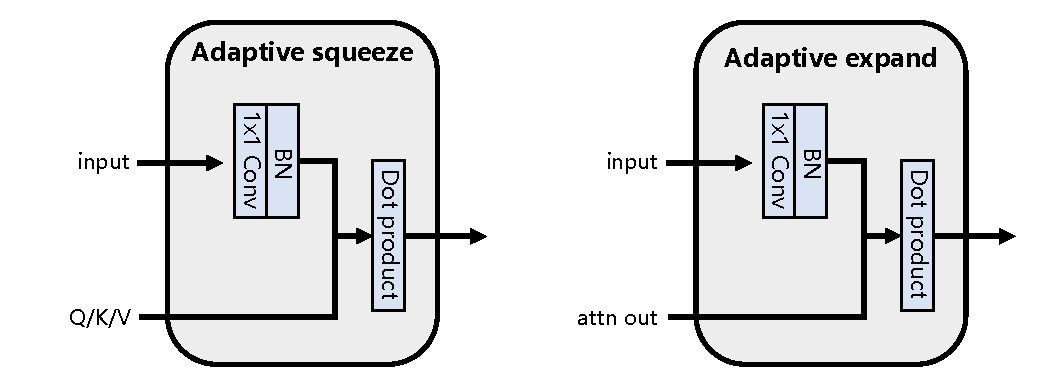
\includegraphics[width=0.8\hsize]{adaptive_sqeeze.pdf}
  \caption{\textit{\textbf{Left}}: the schematic diagram of the proposed adaptive squeezing.
  \textit{\textbf{Right}} is the adaptive expanding operation. \textit{Mat mul} means matrix multiplication. \textit{Attn out} is the output of the multi-head attention.
  }
  \label{fig:squeeze_expand}
  % \vspace{-0.2cm}
\end{figure}
\subsubsection{Complexity analysis}
In our application, we set $C_{qk} = 0.5C_v$ to further reduce computation cost.
The total time complexity of squeeze-enhanced Axial attention is 
\begin{equation}
\begin{split}
    \notag&\mathcal{O}((H^2+W^2)(C_{qk}+C_v) + \mathcal{O}(2HW(2C_{qk} + C_v)) \\
    &+ \mathcal{O}((HWC+9HW)(2C_{qk}+C_{v})) \\
    &=\mathcal{O}((1.5H^2+1.5W^2+4HW)C_v) \\ 
    &+ \mathcal{O}((2HWC+18HW)C_v) \\
    &=\mathcal{O}(HW)
\end{split}
\end{equation}
if we assume $H=W$ and take the channel as constant. SEA attention is linear to the feature map size theoretically.
Moreover, SEA Attention only includes mobile-friendly operations like convolution, pooling, matrix multiplication and so on.

\subsubsection{Architecture details and variants}
SeaFormer backbone contains 6 stages, corresponding to the shared STEM and context branch in Figure 2 in the main paper. When conducting the image classification experiments, a pooling layer and a linear layer are added at the end of the context branch.

Table~\ref{model_var} details the family of our SeaFormer configurations with varying capacities.
We construct SeaFormer-Tiny, SeaFormer-Small,  SeaFormer-Base and SeaFormer-Large models with different scales via varying the number of SeaFormer layers and the feature dimensions. 
We use input image size of $512 \times 512$ by default. 
For variants except SeaFormer-Large, SeaFormer layers are applied in the last two stages for a superior trade-off between accuracy and efficiency. 
For SeaFormer-Large, we apply the proposed SeaFormer layers in each stage of the context branch.
\begin{figure*}
  % \vspace{-0.7cm}
  \centering
  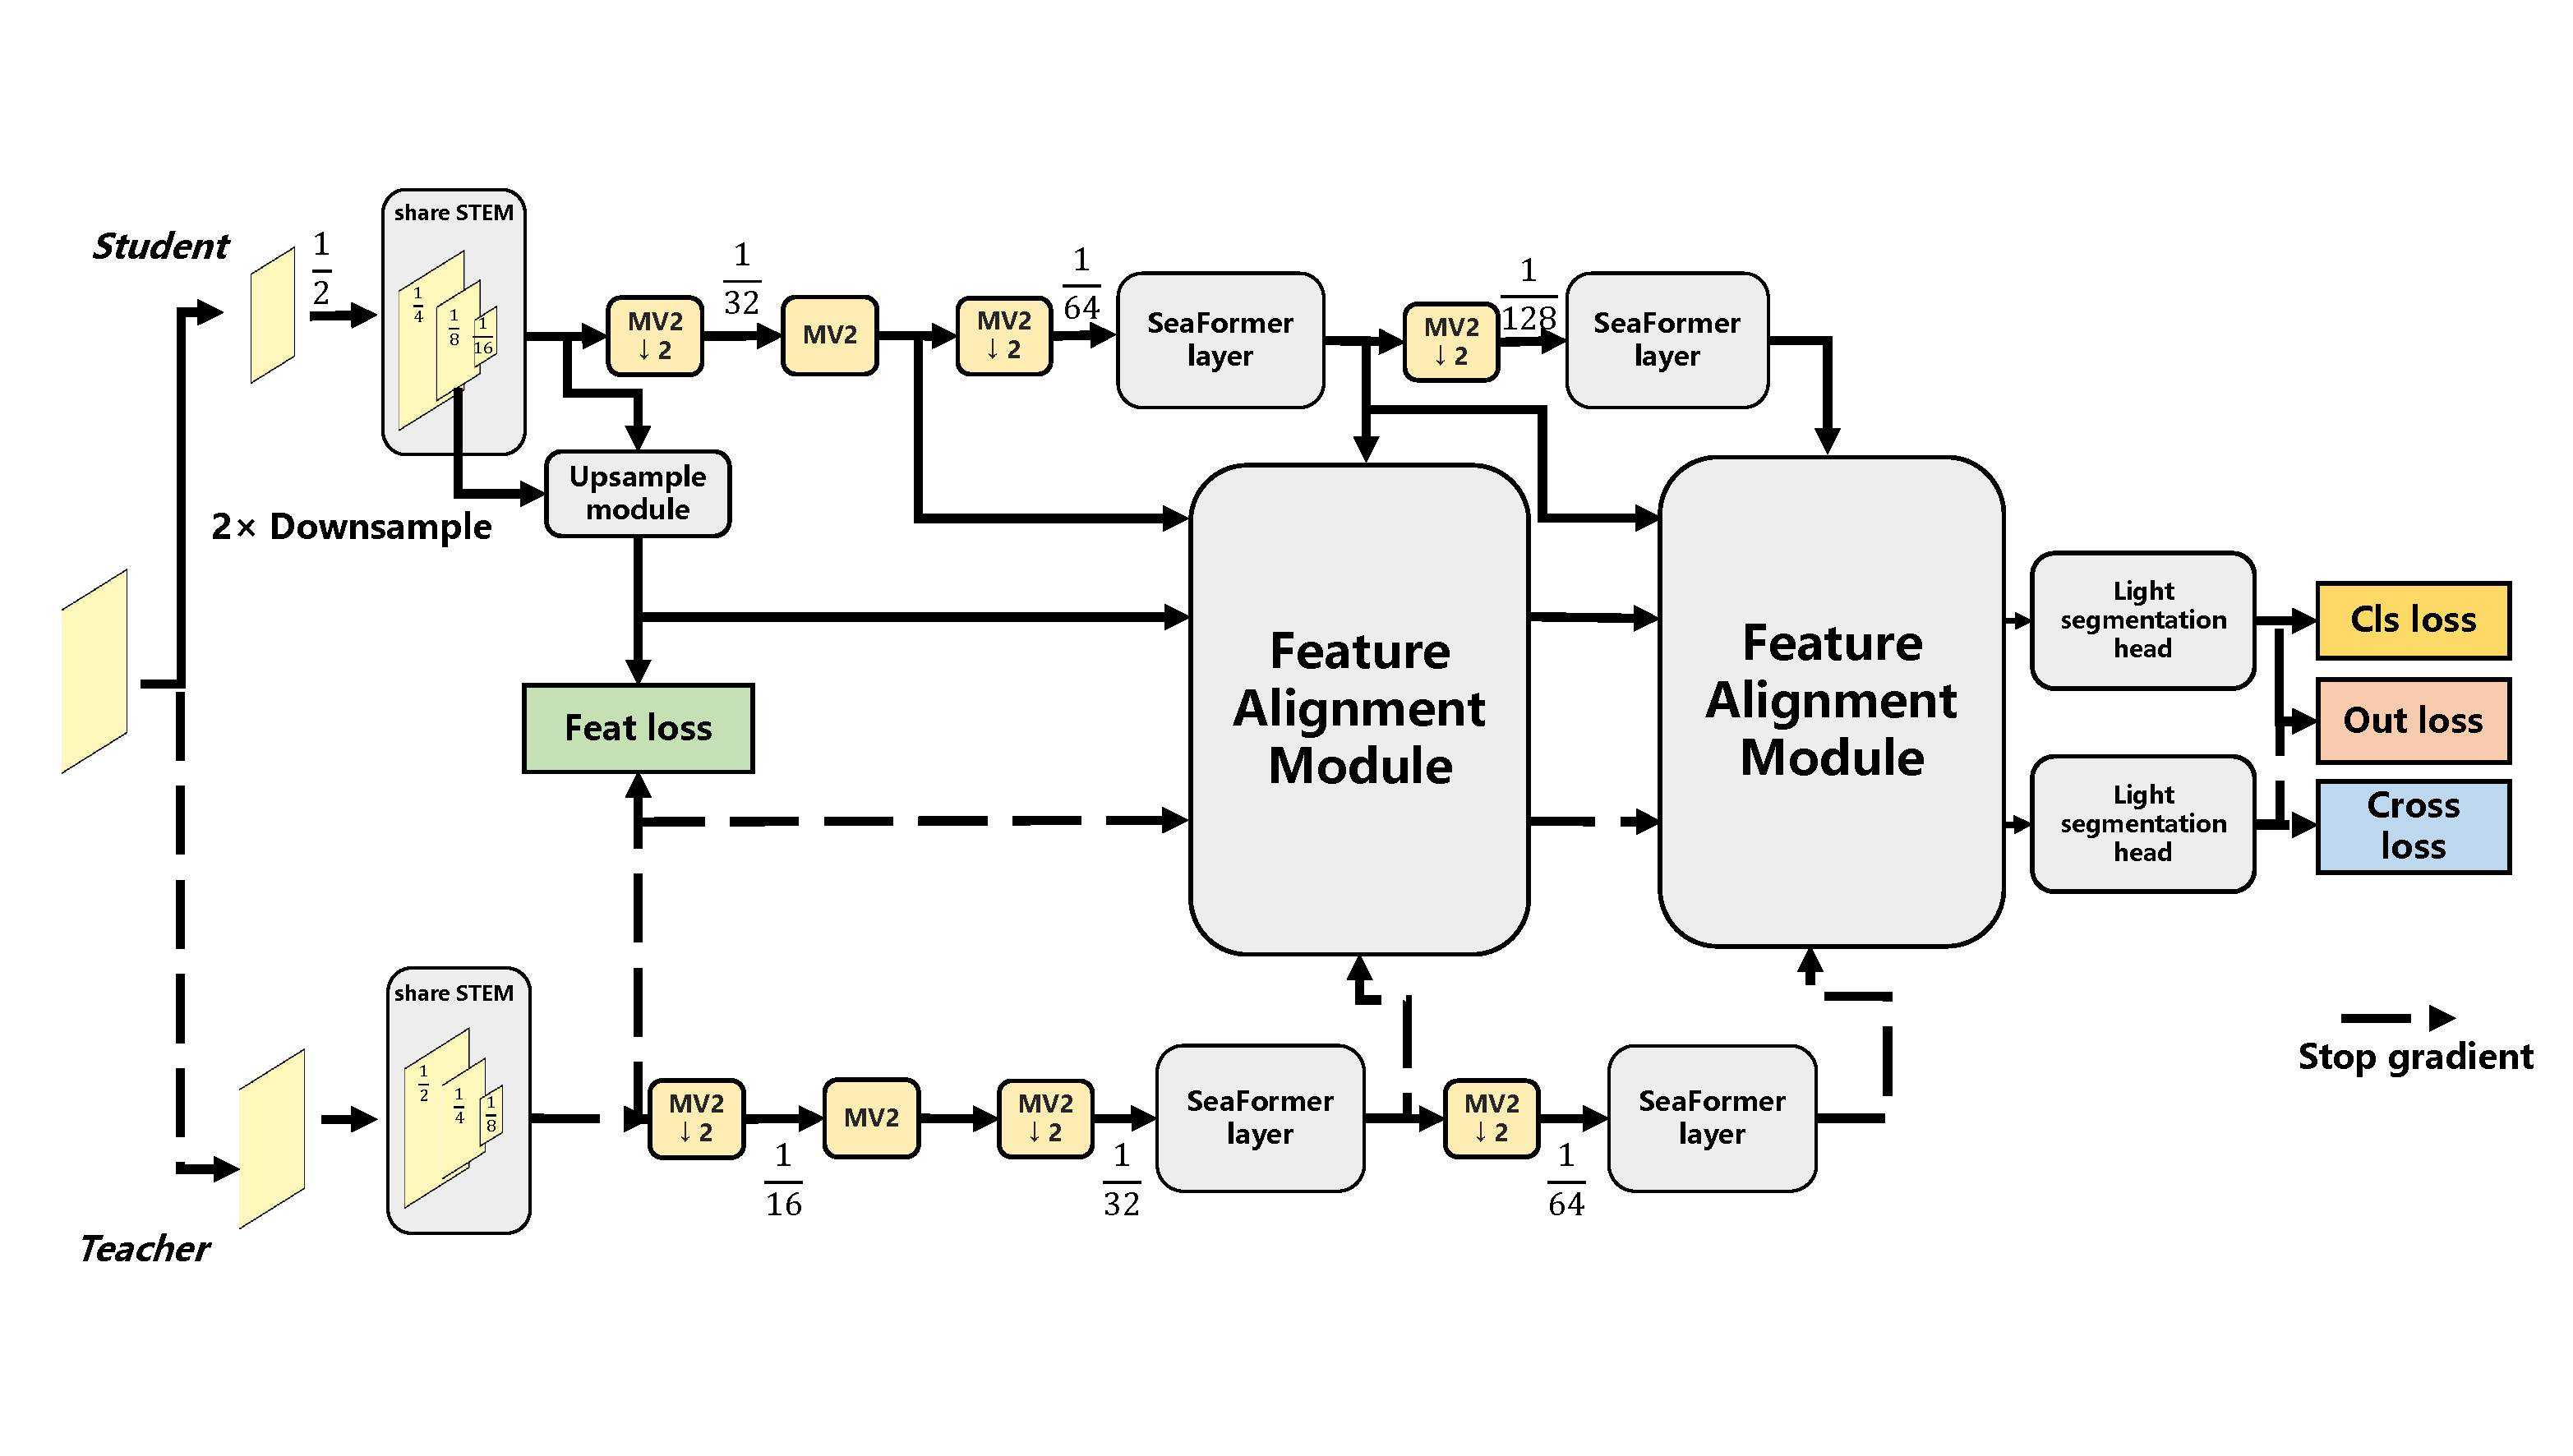
\includegraphics[width=\hsize]{distill_pipeline_.pdf}
  \caption{The overall pipeline of multi-resolution distillation based on feature up-sampling. \texttt{Fusion block} and \texttt{light segmentation head} are consistent with those in Figure~\ref{fig:pipeline}. \texttt{MV2(E=4)} denotes MobileNetV2 block with expansion ratio of 4, and the default kernel size for depth-wise convolution is 5. 
  }
  \label{fig:distill_pipeline}
  % \vspace{-0.2cm}
\end{figure*}
\begin{table*}
\small

  \centering
  \resizebox{1\textwidth}{!}{
  \begin{tabular}{c | c |c  c  c c}
    \hline

    \hline

    \hline
    & Resolution & SeaFormer-Tiny & SeaFormer-Small & SeaFormer-Base & SeaFormer-Large\\
    \hline
    
    \hline
    \hline
    % \hline
    \multirow{2}*{Stage1} & \multirow{2}*{H/2 × W/2} & [Conv, 3, 16, 2] & [Conv, 3, 16, 2] & [Conv, 3, 16,  2]& [Conv, 3, 32, 2] \\
      & & [MB, 3, 1, 16, 1] & [MB, 3, 1, 16, 1] & [MB, 3, 1, 16, 1] & [MB, 3, 3, 32, 1]\\
     \hline
     \multirow{2}*{Stage2} & \multirow{2}*{H/4 × W/4}  
      & [MB, 3, 4, 16, 2] & [MB, 3, 4, 24, 2] & [MB, 3, 4, 32, 2] & [MB, 3, 4, 64, 2]\\
      & & [MB, 3, 3, 16, 1] & [MB, 3, 3, 24, 1] & [MB, 3, 3, 32, 1] & [MB, 3, 4, 64, 1] \\
    \hline
     \multirow{2}*{Stage3} & \multirow{2}*{H/8 × W/8}  
     & [MB, 5, 3, 32, 2] & [MB, 5, 3, 48, 2] & [MB, 5, 3, 64, 2] & [MB, 5, 4, 128, 2] \\
     & & [MB, 5, 3, 32, 1] & [MB, 5, 3, 48, 1] & [MB, 5, 3, 64, 1] & [MB, 5, 4, 128, 1]\\
	\hline
     \multirow{3}*{Stage4} & \multirow{3}*{H/16 × W/16}  
     & [MB, 3, 3, 64, 2] & [MB, 3, 3, 96, 2] & [MB, 3, 3, 128, 2] & [MB, 3, 4, 192, 2]\\
     & & [MB, 3, 3, 64, 1] & [MB, 3, 3, 96, 1] & [MB, 3, 3, 128, 1] & [MB, 3, 4, 192, 1]\\
     & & & & & [Sea, 3, 8] \\
     \hline
     \multirow{2}*{Stage5} & \multirow{2}*{H/32 × W/32}  
     & [MB, 5, 3, 128, 2] & [MB, 5, 4, 160, 2] & [MB, 5, 4, 192, 2] & [MB, 5, 4, 256, 2]\\
     & & [Sea, 2, 4] & [Sea, 3, 6] & [Sea, 4, 8] & [Sea, 3, 8]\\
     \hline
     \multirow{2}*{Stage6} & \multirow{2}*{H/64 × W/64}  
     & [MB, 3, 6, 160, 2] & [MB, 3, 6, 192, 2] & [MB, 3, 6, 256, 2] & [MB, 3, 6, 320, 2]\\
     & & [Sea, 2, 4] & [Sea, 3, 6] & [Sea, 4, 8] & [Sea, 3, 8]\\
\hline

\hline

\hline
  \end{tabular}
  }
  \caption{Architectures for semantic segmentation. [Conv, 3 ,16, 2] denotes regular convolution layer with kernel of 3, output channel of 16 and stride of 2. [MB, 3, 4, 16, 2] means MobileNetV2~\cite{sandler2018mobilenetv2} block with kernel of 3, expansion ratio of 4, output channel of 16 and stride of 2. [Sea, 2, 4] refers to SeaFormer layers with number of layers of 2 and heads of 4.}
  \label{model_var}
\end{table*}




\subsection{Multi-resolution distillation based on feature up-sampling}

In dealing with dense prediction tasks, accurately extracting semantic information and spatial details from images often necessitates the input of high-resolution images. This approach undoubtedly increases the computational burden on the model, especially in resource-constrained environments such as mobile devices or real-time applications, where the demand for high computation becomes even more significant. In recent years, to alleviate this issue, some research~\cite{qi2021multi, hu2022cross} has proposed methods utilizing multi-scale distillation techniques. In these methods, a teacher model that takes high-resolution images as input is used to guide a student model that takes low-resolution images as input to learn. This strategy allows the student model to produce reasonable results even with low-resolution inputs, thereby significantly reducing computational costs and increasing inference speed.

Inspired by the aforementioned methods, this paper proposes an innovative multi-resolution distillation approach based on feature upsampling. Unlike previous work, our method involves aligning the features of the teacher and student models at the same processing stage (even though the student model's input resolution is half that of the teacher model) and particularly emphasizes upsampling at the feature level to achieve alignment.

Specifically, assuming the student model's input resolution is half that of the teacher model, the resolution of the feature maps produced by the student model at any given forward propagation stage will naturally be half that of the corresponding stage in the teacher model. To address this mismatch, this study has designed a feature alignment module. This module employs a lightweight feature upsampling module constructed using MobileNetV2 to upsampling the student model's feature maps to the same resolution as that of the teacher model at the same stage. Subsequently, a feature similarity loss function is used to optimize the similarity between these two features, maximizing their consistency to better aid the student model in mimicking the behavior of the teacher model.

Furthermore, the upscaled features from the student model are not only used for alignment with the teacher model's features but are also integrated into the overall semantic segmentation framework, serving as spatial branch features in the feature fusion process. The specific method of this feature fusion and the involved modules will be detailed in Section~\ref{sec:method}. Through this series of steps, the fused features are finally fed into a lightweight segmentation head to complete the semantic segmentation task.

\subsection{Feature alignment module}
\begin{figure}[ht]
  \centering
  \subfloat[The schematic diagram of the feature alignment module.]{%
    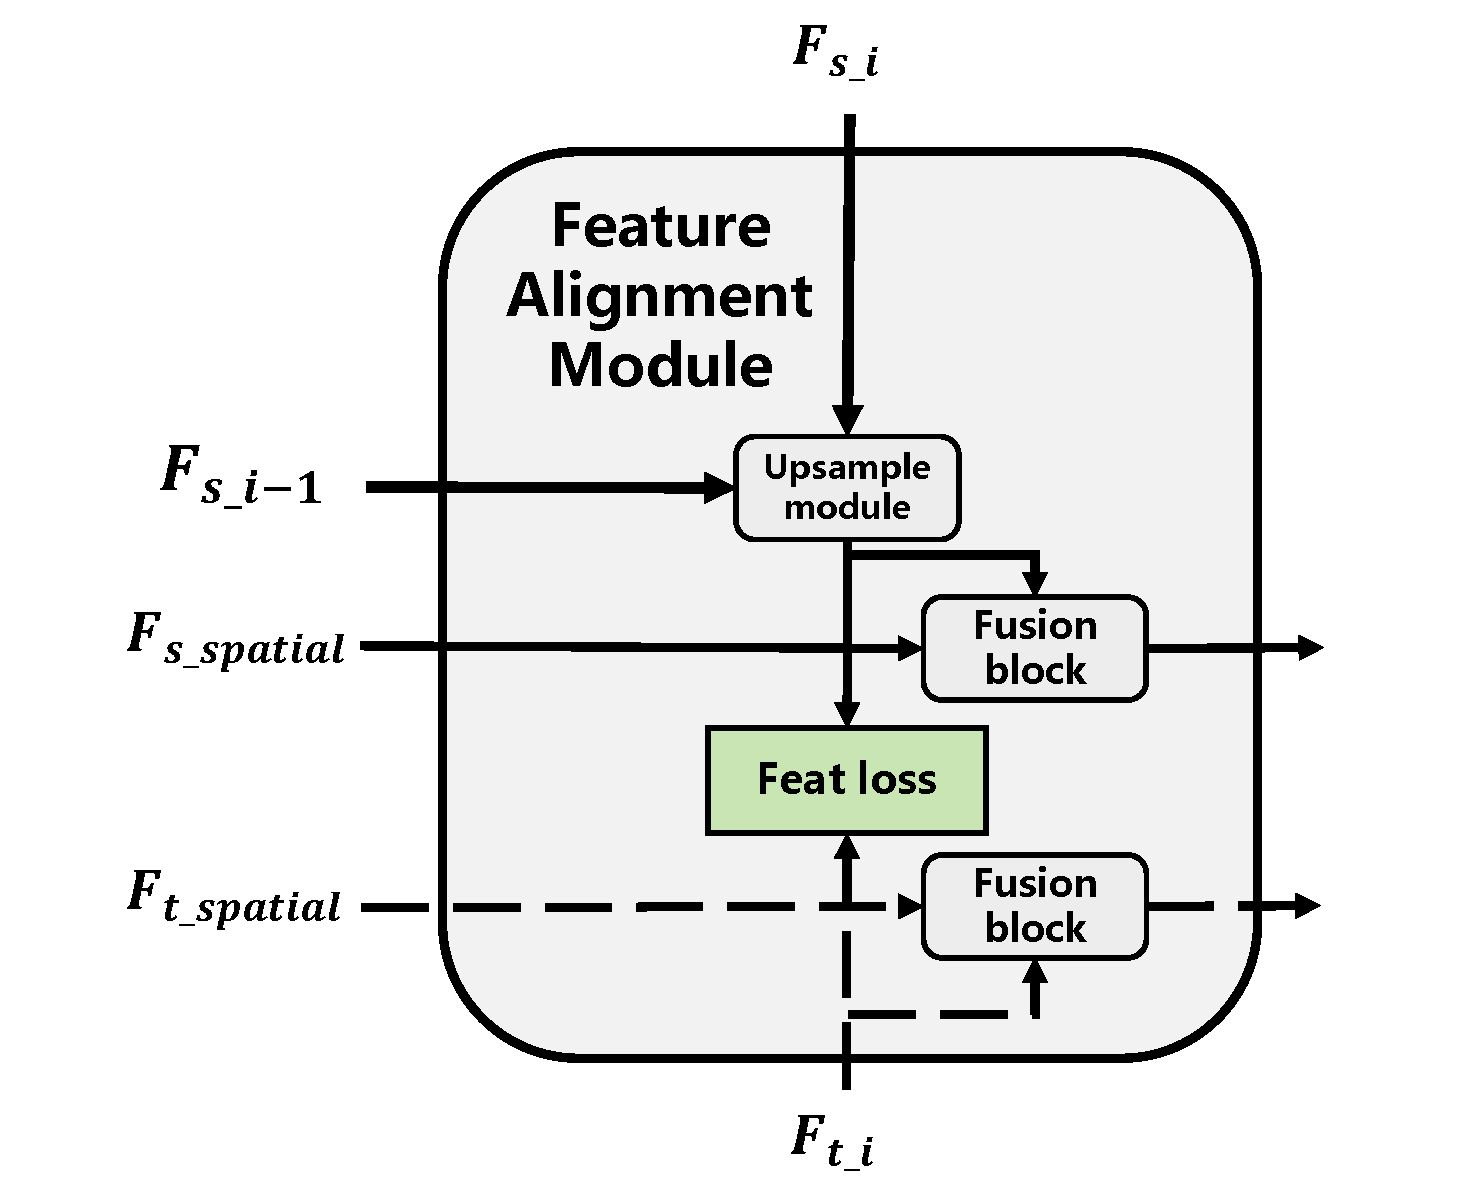
\includegraphics[width=0.45\linewidth]{feature_align_.pdf}%
    \label{fig:feat_align}%
  }
  \quad % 根据需要添加一些水平间隔
  \subfloat[The schematic diagram of the upsample module.]{%
    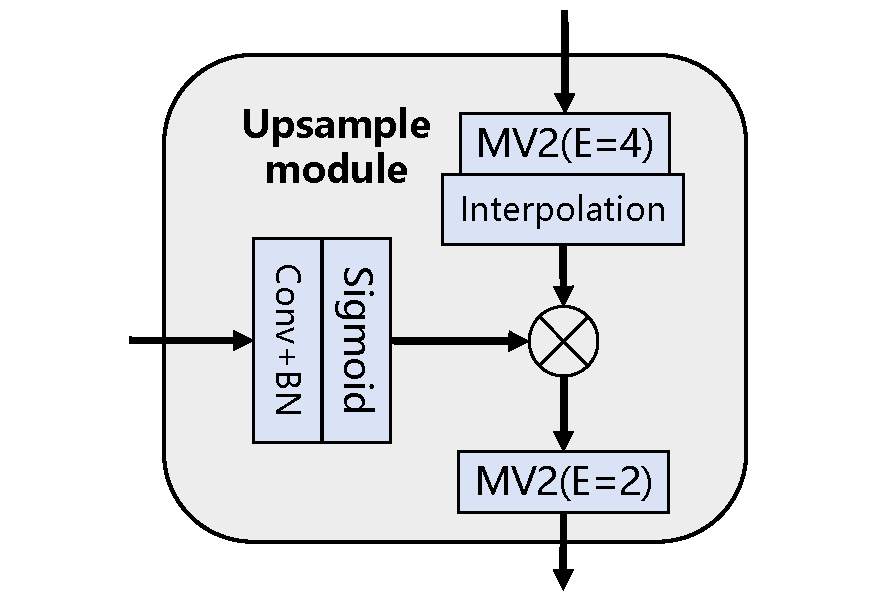
\includegraphics[width=0.45\linewidth]{upsample.pdf}%
    \label{fig:upsample}%
  }
   \caption{\textit{\textbf{Left}}: the schematic illustration of the proposed feature alignment module including an upsample module and a fusion block. \textit{$F_{s\_i}$} means feature map of student model on stage \textit{i}. \textit{$F_{t\_i}$} means feature map of teacher model on stage \textit{i}. \textit{$F_{s\_spatial}$} means feature map of student spatial branch. \textit{$F_{t\_spatial}$} means feature map of teacher spatial branch.
  \textit{\textbf{Right}} is the upsample module.}
  \label{fig:feat_align_upsample}
\end{figure}

Figure~\ref{fig:feat_align} shows the feature alignment module's goal to precisely align the student model's features with the teacher model's, maintaining architectural consistency as described in Section~\ref{sec:method}. This includes using feature fusion to merge spatial and current stage features, and employing the teacher's features as guides to improve the student's feature alignment and predictive accuracy. Initially, the student model's input resolution is halved via average pooling. To address this, a lightweight upsampling module, informed by the detailed matching features of both models, upsamples the student's features for alignment. Cosine similarity between the upscaled and teacher's features, with negative similarity contributing to the loss function, enhances the student's emulation of the teacher's features, ensuring efficient and accurate model performance despite lower input resolution.

\subsubsection{Upsampling module}
Before alignment, the features of the student model are upsampled by applying a lightweight up-sampling module, which ensures that the feature resolution matches the feature resolution of the teacher model at the same stage, facilitating knowledge transfer and improving the performance of the student model. As demonstrated in Figure~\ref{fig:distill_pipeline}, high-resolution feature maps from the previous stage are followed by a convolution, a batch normalization layer, and a sigmoid layer to produce weights to guide the up-sampling of low-resolution features in the current stage. 
Low-resolution feature maps are fed into a  MobileNetV2 block and up-sampled to high resolution.
Then, they are element-wise multiplied with each other, and the up-sampled features are refined with another MobileNetV2 block.

\subsubsection{Loss function}
As indicated in equation~\ref{eqa:distill_loss}, the loss function of the multi-resolution distillation method based on feature up-sampling comprises four components: classification loss, cross-model classification loss, feature similarity loss, and output similarity loss.
\begin{equation}
\begin{split}
\label{eqa:distill_loss}
\mathcal{L}=\mathcal{L}_{cls}+\mathcal{L}_{cross}+\mathcal{L}_{feat}+\mathcal{L}_{out} \\ 
\end{split}
\end{equation}

{\bf Classification loss} $\mathcal{L}_{cls}$ refers to the cross-entropy loss between the output of the student model and the ground truth labels. 

{\bf Cross-model classification loss} $\mathcal{L}_{cross}$ denotes the cross-entropy loss between the output obtained by inputting the up-sampled features of the student model into the segmentation head of the teacher model and the ground truth labels. 

The {\bf feature similarity loss} $\mathcal{L}_{feat}$ measures the negative cosine similarity between the up-sampled features of the student model and the features of the teacher model at the corresponding stage. 

The {\bf output similarity loss} $\mathcal{L}_{out}$ represents the Kullback-Leibler Divergence between the output logits of the student model and the output logits of the teacher model.

The cross-model loss, feature similarity loss, and output similarity loss all contribute to the process of knowledge distillation. Although they differ in terms of the emphasis on the transmitted knowledge from the teacher model to the student model and the degree of relaxation in guiding model parameter updates, they all positively impact the learning of the student model. Our empirical study validates the effectiveness of the aforementioned loss functions.
